\documentclass[%
			%fontsize=12pt,%
			paper=a4,% 
			%DIV12, % mehr text pro seite als defaultyyp
			DIV12,
			%DIV=calc,%
			%twoside=false,%
			liststotoc,
			bibtotoc,
			draft=false,% final|draft % draft ist platzsparender (kein code, bilder..)
			titlepage,
			numbers=noendperiod
			]{scrartcl}


\usepackage[utf8]{inputenc}
\usepackage[T1]{fontenc}
\usepackage[ngerman]{babel}

% for color-highlighted code
\usepackage[usenames]{color} % for grey comments
%\usepackage{alltt}

\usepackage[doublespacing]{setspace}
\usepackage{tabularx}
\usepackage{comment}
\usepackage{color}
\usepackage[final]{listings} % sourcecode in document
\usepackage{url}      % for urls
\usepackage{multicol}
\usepackage{caption}
\usepackage{subfigure}
\usepackage{enumerate}

\usepackage{graphicx}

%\usepackage[square]{natbib} % \cite ; square|round etc.
\usepackage[numbers,square]{natbib}
%\usepackage[square, authoryear]{natbib}

%\usepackage{bibgerm}
%\bibliographystyle{plain}
%\bibliographystyle{alpha}
\bibliographystyle{alphadin}
%\bibliographystyle{dinat}
%\bibliographystyle{chicago}
%\bibliographystyle{plainnat}

%\bibdata{bib.bib}

\newcommand{\zit}[3]{#1 \cite{#2}, #3}
\newcommand{\zitx}[2]{#1 \cite{#2}}
\newcommand{\footzit}[3]{\footnote{\zit{#1}{#2}{#3}}}
\newcommand{\footzitx}[2]{\footnote{\zitx{#1}{#2}}}

\newcommand{\footurl}[2]{\footnote{\url{#1}, abgerufen am #2}}

\newcommand{\inlinecode}[1]{\mbox{\texttt{#1}}}

\newcommand{\mynull}{\textit{NULL}}
%\newcommand{\mynull}{\textbf{nil}}

\newcommand{\kd}{\mbox{\textit{k}-d}}

\renewcommand*{\partformat}{\partname\ \thepart\ -}
\let\partheadmidvskip\



% smaller url style
\makeatletter
\def\url@leostyle{%
\@ifundefined{selectfont}{\def\UrlFont{\sf}}{\def\UrlFont{\small\ttfamily}}}
\makeatother
\urlstyle{leo}

\newcommand{\myfig}[5] {
 \begin{figure}[tbph]
	 \centering
	 \includegraphics[#3]{#1}
	 \caption[#4]{#5}
	 \label{fig:#2}
 \end{figure}
}

\title{Quadtrees}
\author{Bernhard Mallinger \\ 0707663 \\ TU Wien}
%\subtitle{}
%\date{13. November 2007}
\publishers{Betreut durch Univ.-Ass. Dipl.-Ing. Christian Schauer, BSc}

%\usepackage{fancyhdr}
%\setlength{\headrulewidth}{0.0pt}
\pagestyle{plain}

\definecolor{grey}{gray}{.35} % for grey commnts
\lstset{language=Python,%
escapeinside={@}{@},
extendedchars=false,%
%inputencoding=utf8x,%
basicstyle=\ttfamily\small,%
commentstyle=\color{grey},%
%keywordstyle=,% no bold tt in standard font
%captionpos=b,
tabsize=2,
showstringspaces=false,
breaklines=true,
breakindent=0pt,
numbers=left
}

% just for screen-display!
%\usepackage{newcent}

\begin{document}

\maketitle

\tableofcontents 

\newpage

%%%%
% TODO
%
% Einleitung mit erklärung:
% k
% n
% schlüssel
% mehrdimensionale daten (bisschen wie kdtree.pdf)
%
% schlüssel unique -- überlauflisten
%
% binäre suche im anfang reinbringen -- bin tree
%
% point qt: suche: neighborhood 
%
% anwendungen (vllt extrakapitel) (kriterien für anwendbarkeit)
%
% seite 3 (aus paper zitieren)
%
% bild pr tree 
%
% kurz erweiterung auf mehrere dimensionen am bsp von octtree besprechen
%
% pr quadtree vllt noch mehr literatur finden


\part{Theorie}

\section{Einführung}
Quadtrees stellen eine Datenstruktur dar, welche von Binärbäumen abgeleitet ist.
Sie erweitern das Binärbaum-Prinzip der rekursiven, hierarchischen Aufteilung eines Raumes auf mehrere Dimensionen. 
Im Allgemeinen beschränkt man sich hier zur Vereinfachung auf zwei- bzw.\ dreidimensionale Daten, wobei die Verallgemeinerung auf \textit{k}-dimensionale Daten trivial ist.\footzit{Vgl}{DBLP:journals/acta/FinkelB74}{Seite 9}

Anstatt wie bei Binärbäumen den Raum in jedem Schritt in einen linken und einen rechten Teilbaum zu zerlegen, werden bei Quadtrees vier Kinder verwendet, um alle möglichen Richtungen (links, rechts, oben, unten) in zwei Dimensionen bezüglich des aktuellen Knotens abzudecken. Der Name "`Quadtree"' leitet sich hiervon ab (lat. "`quadri-"': "`vier-"'). 
Analog dazu bezeichnet man dreidimensionale Bäume als "`Octtrees"'. Es ist weiters einfach zu sehen, dass $k$-dimensionale Bäume $2^k$ Kinder pro Knoten aufweisen.\footzit{Vgl.}{Bentley:1979}{Seite 16}

Räumliche Strukturen wie Quadtrees sind generell dann sinnvoll, wenn die Entfernung zweier Punkte für die Anwendung relevant ist.
Beispiele hierfür sind unter anderem die Repräsentation von Bildern (angrenzende Bereiche besitzen oftmals ähnliche Farben), Kollisionserkennung (wo das Interesse auf sich überschneidenden Strukturen liegt), oder Bereichsabfragen in Datenbanken.

Beim Zugriff auf die so in einem Quadtree gespeicherten Daten unterscheidet man zwischen verschiedenen Anfragetypen:\footnote{Basierend auf \cite{Knuth:1998:ACP:280635}, Seite 559 und der Erweiterung durch \cite{Bentley:1975:nearest}}
\begin{description}
	\item[Point Query.]
		Mit dieser Anfrage versucht man herauszufinden, welche Daten sich an einem bestimmten Punkt befinden.
		Antworten auf diese Anfrage können entweder ein Datenobjekt oder \mynull\ sein.
	\item[Range Query.]
		Hier interessiert man sich für die Knoten, welche innerhalb von Bereichen liegen, die hinsichtlich mehrerer Dimensionen ausgedehnt sein können.
		Zurückgegeben wird eine möglicherweise leere Liste von Datenobjekten.
	\item[Neighborhood Query.]
		Dieser Anfragetyp fokussiert sich auf Nähebeziehungen.
		Konkret werden die Knoten gesucht, welche die geringste Entfernung zu einem bestimmten Knoten aufweisen oder sich innerhalb eines gewissen Radius davon befinden.
		Der Rückgabewert kann hier eine Liste oder ein einzelnes Datenobjekt sein.
\end{description}


\subsection{Funktionsprinzip}

Wie eingangs erwähnt, wird bei einem Quadtree der Raum in jedem Schritt in zwei Dimensionen geteilt.
In diesem Kontext bezeichnet man die Abschnitte der Unterteilung als "`Quadranten"'.
Diese Aufteilung kann, wie Abbildung \ref{fig:quadtree} demonstriert, direkt am Knoten stattfinden, je nach Quadtreetyp werden hier jedoch verschiedene Strategien eingesetzt.

Die eigentlichen Daten werden je nach Quadtreetyp in allen Knoten oder nur den Blättern gespeichert.
Alle Knoten eines Baumes beinhalten zusätzlich Verweise auf vier Teilbäume, welche diejenigen Daten beinhalten, die sich jeweils vollständig in der entsprechenden Richtung des Elternknotens befinden. 
Die Koordinaten der zu speichernden Daten bestimmen demnach die Struktur des Quadtrees.

Dieses Prinzip der rekursiven, hierarchischen Dekomposition erlaubt das effiziente Suchen in logarithmischer Zeit, sofern eine adäquate Balancierung sichergestellt ist.\footnote{Siehe Kapitel \ref{sec:pointquadtree-suche}}
\myfig{img/quadtree}{quadtree}{width=.6\textwidth}{Funktionsprinzip eines Quadtrees}{Alle Kinder eines Knotens repräsentieren Teilbäume, welche sich vollständig in NW-, NE-, \mbox{SW-} oder SE-Richtung des aktuellen Knotens befinden. Je nach Konvention können die Quadranten auch mittels ihrer Nummerierung referenziert werden. Diese Darstellungsform wird im Folgenden als Koordinatendarstellung bezeichnet.}

\section{Punktbasierte Quadtrees}
\label{sec:pointbased}
\subsection{Point Quadtree}
Dieser Quadtreetyp wurde erstmals 1974 von Finkel und Bentley in \cite{DBLP:journals/acta/FinkelB74} eingeführt und stellt die Basis vieler weiterer Entwicklungen dar.\footzit{Vgl.}{compgeom:2000}{Seite 318}
Point Quadtrees kann man als direkte Verallgemeinerung von binären Suchbäumen auf mehrdimensionale Räume auffassen.\footzit{Vgl.}{Samet90}{Seite 48}
Ähnlich zu diesen Bäumen erfolgt die Aufteilung direkt an den Koordinaten der Knoten, sowie an beiden Dimensionen gleichzeitig. 

% vllt deBerg S 316 tiefe O( (d+1) n )
% und S 322
% As we have seen in this chapter, the size and depth of a quadtree for a set of n points cannot be bounded in terms of the number of the number of points only.

Abbildung \ref{fig:pointquadtree} zeigt eine Instanz eines Point Quadtrees in zwei üblichen Darstellungsvarianten: Baum- und Graphenform.
In der ersten Variante wird nur die Struktur des Baumes betrachtet, die Lage der Datenknoten ist ausschließlich relativ zueinander sichtbar.
Die zweitere konzentriert sich mehr auf die absolute Position der Punkte in einem Koordinatensystem und zeigt zusätzlich dazu die rekursive Dekompositionsstruktur an.
Die Bezeichnung der Knoten in der Grafik gibt hier die Reihenfolge des Einfügens an. Bereits hier wird deutlich, dass die Form des Baumes durch diese Reihenfolge determiniert wird.\footnote{Vgl. Kapitel \ref{sec:pointquadtree:insert}}
\myfig{img/pointquadtree-ins7+tree-trimmed}{pointquadtree}{width=.9\textwidth}{Point Quadtree}{Gegenüberstellung: ein Point Quadtree in Baum- bzw.\ Koordinatendarstellung}

\subsubsection{Suche}
\label{sec:pointquadtree-suche}
Der Algorithmus zur Suche von Knoten (Point Query) ergibt sich unmittelbar aus dem rekursiven Aufbauprinzip des Quadtrees. 

Die Suche beginnt an der Wurzel. In jedem Schritt werden je ein Vergleich der $x$- und $y$-Koordinate des aktuellen Knotens mit dem gesuchten Knoten durchgeführt, wodurch der Quadrant bestimmt wird, in welchem sich der gesuchte Knoten befindet.
Ist dieser Quadrant leer, d.h.\ ist kein Kindknoten bezüglich dieser Richtung vom aktuellen Knoten ausgehend vorhanden, wird die Suche erfolglos abgebrochen; andernfalls wird sie bei dem Kindknoten, welcher diesen Quadranten abdeckt, rekursiv fortgesetzt, bis die Koordinaten des gesuchten Knotens mit jenen des aktuellen Knoten übereinstimmen.

Durch die rekursive Aufteilung kann bei $N$ Knoten nach dem Erstellen des Quadtrees mit einer Gesamtpfadlänge\footnote{engl. TPL: Total path length, d.h. die Summe der Längen aller Pfade im Baum} von
$O(N \log_4 N)$ gerechnet werden,
was in empirischen Untersuchungen mit Einfügungen in zufälliger Reihenfolge bestätigt wurde.\footzit{Vgl.}{DBLP:journals/acta/FinkelB74}{Seite 4}
Dies führt in der Folge bei der Suche nach einzelnen Punkten zu einer Laufzeit von $O(\log_4 N)$.
Allerdings hängt diese Größe von der Balancierung des Baumes ab, wofür es beim Point Quadtree keine Garantien gibt,\footnote{Vgl. Kapitel \ref{sec:pointquadtree:insert}}
was im Falle einer Entartung (Worst Case) zu einer linearen Laufzeit von $O(N)$ führt.\footzit{Vgl.}{Samet90}{Seite 52}

Die Bereichssuche gestaltet sich ähnlich der Punktabfrage.
Der essentielle Unterschied besteht darin, dass hier die Suche möglicherweise in mehreren Quadranten eines Knotens fortgesetzt werden muss.
Die zu durchsuchenden Quadranten werden bestimmt, indem überprüft wird, ob der Bereich dieses Quadranten mit dem gesuchten Bereich überlappt.
Weiters wird für jeden Knoten, welcher besucht wird, festgestellt, ob er sich in dem spezifizierten Bereich befindet; dieser wird gegebenenfalls zurückgegeben.\footzit{Vgl.}{DBLP:journals/acta/FinkelB74}{Seite 5f}
In dieser Formulierung wird ebenso sofort deutlich, dass die gesuchte Region nicht unbedingt ein Rechteck bilden muss.

%Weiters kann gezeigt werden, dass Range Queries in $O(n\ log_k\ n)$ abgearbeitet werden können.\footzit{Vgl.}{Lueker78}{Seite 1}

\subsubsection{Einfügen}
\label{sec:pointquadtree:insert}
Das Verfahren zum Einfügen neuer Daten baut direkt auf der Suche auf.
%In dem Quadranten, in welchem eine normale Suche abbrechen würde, wird das Datum eingefügt, indem an der entsprechenden Stelle, die sich offensichtlicher Weise in diesem Quadranten befinden muss, der Datenknoten platziert wird.
Das heißt, man sucht nach dem einzufügenden Objekt und findet dieses nicht.
Anstatt nun aber zu terminieren, wird an der potentiell freien Stelle das entsprechende Objekt hinzugefügt.
Konkret geschieht dies durch Setzen des diesem Quadranten zugeordneten Zeigers im Elternknoten.
Der asymptotische Aufwand dieser Operation ist natürlich identisch mit jenem der Suche.

Der neu eingefügte Knoten teilt den Raum wiederum an seinen $x$- bzw. $y$-Koordinaten und erweitert so die Struktur des Baumes.  
Es ist schnell ersichtlich, dass hier, genau wie bei einem Binärbaum, Entartungen auftreten können, da sich die Struktur dynamisch mit jedem eingefügten Element herausbildet.

Ein besonderes Problem stellen hier etwa geordnete Daten da. Werden diese in der gegebenen Reihenfolge eingefügt, degeneriert der Baum zu einer linearen Liste, wodurch ein linearer Such- und somit gleichzeitig auch Einfügeaufwand entsteht, wie Abbildung \ref{fig:entartung} demonstriert.
\myfig{img/pointquadtree-entartet-trimmed}{entartung}{width=.6\textwidth}{Entarteter Point Quadtree}{Ein entarteter Point Quadtree}

Sind andererseits beim Aufbau des Baumes bereits alle Daten verfügbar, kann durch folgende Strategie eine optimale Balancierung erreicht werden: Der Median der sortierten Liste von Daten wird als Wurzel verwendet, die restlichen Elemente werden in 4 Gruppen eingeteilt, welche den Quadranten dieser Wurzel zugeordnet werden.
Auf jede dieser Unterteilungen wird der Prozess rekursiv angewendet. Dadurch kann erreicht werden, dass für jeden Knoten kein Kind mehr als die Hälfte aller Subknoten von diesem enthält, was empirisch zu 15\% geringeren Gesamtpfadlängen führt.\footzit{Vgl.}{DBLP:journals/acta/FinkelB74}{Seite 8f}


\subsubsection{Löschen}
\label{sec:pointquadtree:delete}
Das Entfernen eines Knotens aus einem Quadtree ist im Allgemeinen eine komplexe Operation, da die Knoten alleine die Struktur des Baumes bilden, und diese auch nach dem Löschen weiterhin gewisse Eigenschaften innehaben muss.
Daher ist es notwendig, eventuelle Kinder eines entfernten Knotens gemäß dem Baumaufbau neu zu platzieren.\footzit{Vgl.}{DBLP:journals/acta/FinkelB74}{Seite 8}
Bei Binärbäumen stellt dies kein allzu großes Problem dar, da in einem eindimensionalen Raum immer ein geeigneter Ersatz in Form des nächsten Knotens für einen zu entfernenden Knoten zur Verfügung steht.\footzit{Vgl.}{DBLP:journals/cacm/Samet80a}{Seite 2}
Im Fall von Quadtrees muss eine Substitution hingegen Bedingungen hinsichtlich zweier Dimensionen genügen, wodurch es ein Näheverhältnis wie im eindimensionalen Fall nicht gibt.\footzit{Vgl.}{DBLP:journals/cacm/Samet80a}{Seite 2}
Hier ist ein Ersatz nur dann möglich, wenn ein Blattknoten existiert, für den sich im Bereich zwischen den Achsen, welche durch die Koordinaten des Blattknotens bzw.\ deren des zu entfernenden Knotens verlaufen, kein anderer Knoten befindet.\footzit{Vgl.}{DBLP:journals/cacm/Samet80a}{Seite 3}

Ursprünglich wurde vorgeschlagen, alle Kinder des zu entfernenden Knotens neu einzufügen, was einen sehr aufwändigen Prozess darstellen kann.\footzit{Vgl.}{DBLP:journals/acta/FinkelB74}{Seite 8}
Sollte kein Knoten das oben genannte Kriterium erfüllen, kann nur durch günstige Wahl des Ersatzknotens die Anzahl der neu einzufügenden Knoten minimiert werden, wie etwa in \cite{DBLP:journals/cacm/Samet80a} gezeigt wird.

Eine weitere Optimierung kann dadurch erreicht werden, dass gelöschte Knoten nicht aus dem Baum entfernt, sondern nur als gelöscht markiert werden, um so die Struktur zu erhalten.
Die markierten Knoten dürfen bei zukünftigen Suchen nicht mehr zurückgegeben werden.
Nach jeder Entfernung erhöht sich hierdurch der Anteil der "`toten"' Knoten, was sich negativ auf die Performance aller Operationen auswirkt und periodische Restrukturierungsmaßnahmen des Baumes erfordert.
Durch dieses Verfahren kann folglich der Aufwand einzelner Löschoperationen abgefedert werden, mit dem Nachteil von regelmäßigen Wartungskosten.

\subsection{Pseudo Quadtree}
\label{sec:pseudoquadtree}
Der Pseudo Quadtree ist eine Abwandlung des Point Quadtrees, welche Löschen in logarithmischer Zeit sowie einfachere Rebalancierung bei Deformation ermöglicht. Diese Form des Quadtrees wurde 1982 von Overmars und van Leeuwen in \cite{DBLP:journals/acta/OvermarsL82} entwickelt.

Dem Pseudo Quadtree liegt die Analyse zu Grunde, dass die Probleme beim Entfernen von Knoten und bei der Balancierung bei Point Quadtrees daher stammen, dass die Datenpunkte selbst die Struktur des Baumes bilden und so nur äußerst wenig Flexibilität vorhanden ist.\footzit{Vgl.}{DBLP:journals/acta/OvermarsL82}{Seite 6}
Der Pseudo Quadtree unterscheidet sich davon insofern, als dass die Dekomposition des Raumes an theoretisch beliebigen Punkten stattfinden kann. 

Konkret funktioniert das Einfügen beim Pseudo Quadtree wie folgt:
Der Quadrant eines Datenpunktes wird gesucht.
Ist dieser leer, wird der Knoten hier eingefügt, ohne den Raum an dessen Koordinaten weiter zu unterteilen.
Befindet sich hier hingegen bereits ein anderer Knoten, muss eine neue Untergliederung eingeführt werden.
Hier können verschiedene Strategien verwendet werden, um einen Teilungspunkt zu bestimmen, wodurch ein der Anwendung angepasster, gut balancierter Baum entstehen kann.
Als einzige Postcondition dieser Strategien muss garantiert werden,
dass die Knoten in verschiedene Quadranten gespeichert werden.\footzit{Vgl.}{DBLP:journals/acta/OvermarsL82}{Seite 6}

Abbildung \ref{fig:pseudoquadtree} zeigt einen Pseudo Quadtree, welcher dieselben Daten wie der Point Quadtree in Abbildung \ref{fig:pointquadtree} beinhaltet.
\myfig{img/pseudoquadtree-ins3-trimmed}{pseudoquadtree}{width=.6\textwidth}{Pseudo Quadtree}{Pseudo Quadtree}

Sollte trotz einer angepassten Strategie ein Ungleichgewicht entstehen, kann der Subbaum, dessen Wurzel der höchste Knoten ist, bei welchem eine unbalancierte Verteilung seiner Kindknoten festgestellt wird, neu strukturiert werden, indem eine neue Aufteilung der vorhandenen Knoten berechnet wird.\footzit{Vgl.}{DBLP:journals/acta/OvermarsL82}{Seite 4f} % cp
Es kann gezeigt werden, dass im allgemeinen Fall eine Teilung möglich ist,
so dass sich in keinem der vier Quadranten mehr als ein Drittel der Knoten befindet.\footzit{Vgl.}{DBLP:journals/acta/OvermarsL82}{Seite 7} % cp
Mit dieser Methode kann weiters garantiert werden, dass ein Pseudo Quadtree aufgebaut werden kann, dessen Höhe $\lceil \log_{d+1} N\rceil$ nicht überschreitet, wobei $N$ die Anzahl der Knoten sowie $d$ die Anzahl der Dimensionen darstellt.\footzit{Vgl.}{DBLP:journals/acta/OvermarsL82}{Seite 8}

Durch Raumaufteilung der Punkte befinden sich Daten schließlich nur noch an den Blättern. Dies wiederum ist der optimale Fall bezüglich des Entfernens von Knoten -- ein Knoten ohne Kinder kann jederzeit ohne zusätzlichen Aufwand gelöscht werden. Da das Entfernen eines Knotens immer auch das Suchen desselben erfordert, entsteht somit ein logarithmischer Aufwand.

%\ref{sec:pointquadtree:delete} 

\subsection{\kd\ Tree}
Diese Variante wurde von Bentley kurz nach dem Point Quadtree 1974 in \cite{Bentley:1975} entwickelt. Der Name \kd\ deutet an, dass dieser Baum $k$-dimensionale Schlüssel verwendet. 

Der \kd\ Tree kann wie der Point Quadtree als Verallgemeinerung des Binärbaums gesehen werden, hier wird hingegen ein etwas anderer Ansatz verfolgt:
Anstatt den Raum auf jeder Teilungsebene in allen Dimensionen zu partitionieren, was zu $2^k$ Kindern pro Knoten führt, wird in jedem Schritt nur eine Dimension berücksichtigt und so eine binäre Unterteilung von eigentlich mehrdimensionalen Schlüsseln ermöglicht.
Diese Mehrdimensionalität wird bei \kd\ Trees weiters dadurch ausgedrückt, dass die Dimensionen, bezüglich derer an einer gewissen Tiefe geteilt wird, nach verschiedenen Strategien alternieren.
Im zweidimensionalen Fall könnte hier etwa bei geraden Tiefenebenen an der $x$-Achse bzw.\ bei ungeraden an der $y$-Achse geteilt werden, wie Abbildung \ref{fig:kdtree} zeigt.
Ursprünglich wurde genau dieses Abwechslungsmuster vorgeschlagen,\footzit{Vgl.}{Bentley:1975}{Seite 2}
wobei es, an die Daten angepasst, dynamisch gewählt werden kann\footzit{Vgl.}{Samet90}{Seite 66}.
Verwendet man hier einen dynamischen Ansatz, muss jedoch bei jedem Knoten der Diskriminator mitgespeichert werden.

\begin{figure}[h]
	\centering
	\subfigure[]{
	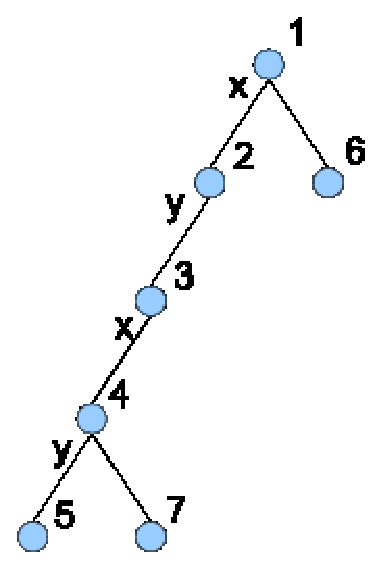
\includegraphics[width=.23\textwidth]{img/kdtree-tree-trimmed}
	\label{fig:kdtree1}
	}
	\hspace{2em}
	\subfigure[]{
	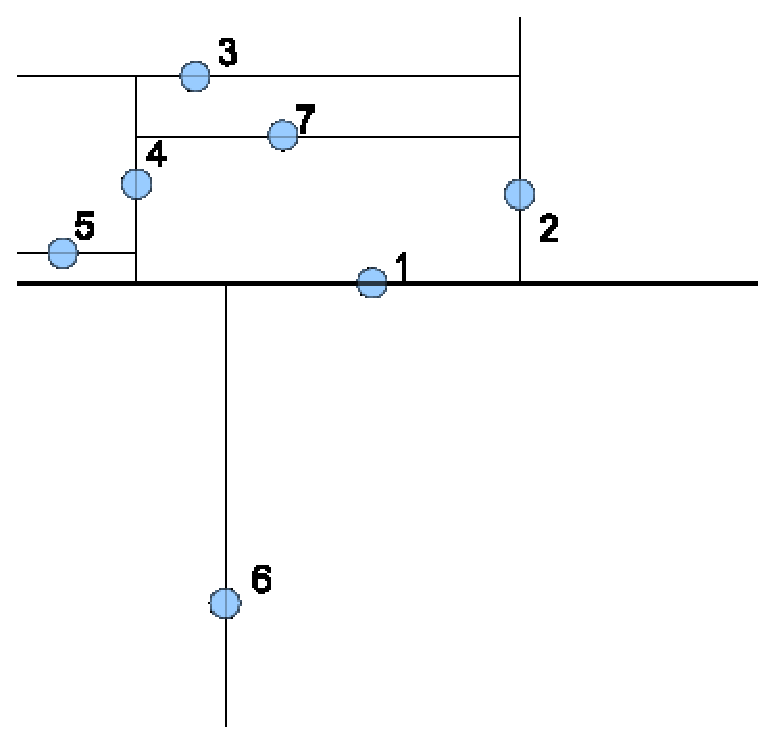
\includegraphics[width=.4\textwidth]{img/kdtree-full-trimmed}
	\label{fig:kdtree2}
	}

	\caption[\kd\ Tree]{Ein \kd\ Tree in Baum- bzw.\ Koordinatendarstellung.
	\\ \\
	(a) Die Beschriftung der Unterteilungen gibt die Achse an, bezüglich welcher die Knoten aufgeteilt werden.
	\\ \\
	(b) Hinsichtlich der vorhergegangenen Abbildungen wurden hier die Koordinaten der Knoten leicht verändert, da in diesem Fall ein äußerst schlecht balancierter \kd\ Tree entstehen würde, was der Autor aus Demonstrationszwecken vermeiden möchte.}
	\label{fig:kdtree}
\end{figure}

%\myfig{img/kdtree-tree-full-trimmed}{kdtree}{width=.78\textwidth}{\kd\ Tree}{Ein \kd\ Tree: Die Beschriftung links der Unterteilungen gibt die Achse an, bezüglich welcher die Knoten aufgeteilt werden.
%\\ \\
%Bezüglich den vorhergegangenen Abbildung wurden hier die Koordinaten der Knoten leicht verändert, da in diesem Fall ein äußerst schlecht balancierter \kd\ Tree entstehen würde, was der Autor aus Demonstrationszwecken vermeiden möchte.}

Dieser Typ bietet gegenüber einem Point Quadtree Vorteile bezüglich des Platzbedarfs:
anstatt $2^k$ sind hier nur 2 Kinder pro Knoten erforderlich.
Dies löst das Problem von vielen unnötigen Leereinträgen, welche bei einem Point Quadtree bei höherdimensionalen Datensätzen auftreten können.

Weiters müssen bei einem Point Quadtree bei einer Suche in jedem Schritt alle Dimensionen verglichen werden.
Bei einer großen Anzahl von Dimensionen kann dies überflüssig sein, wenn sich etwa Datensätze bereits durch eine echte Teilmenge ihrer Schlüssel einteilen lassen.
In diesem Fall reicht das Überprüfen dieser Teilmenge,
was in einem Point Quadtree nicht realisierbar ist, sich mit dem \kd\ Tree jedoch effizient verwirklichen lässt.\footzit{Vgl}{Samet90}{Seite 66}

Die Operationen Suchen und Einfügen ergeben sich direkt aus dem Funktionsprinzip des \kd\ Trees, beide benötigen offensichtlich eine logarithmische Laufzeit im Average Case\footzit{Vgl.}{Bentley:1975}{Seite 1} (sofern der Baum nicht entartet).
Schwieriger ist hingegen das Löschen:
Nach dem Entfernen eines Knotens darf die Struktur des \kd\ Trees nicht verletzt werden, weshalb ein geeigneter Ersatz gefunden werden muss.
Für dieses Problem wurde eine Strategie entwickelt, welche auf der Lösung des analogen Problems bei Binärbäumen basiert und zugleich die Mehrdimensionalität im \kd\ Tree berücksichtigt.
Der wesentliche Aspekt dieses Verfahrens ist, dass der Ersatzknoten nicht wie beim Binärbaum immer ein Blatt ist, sondern im Allgemeinen auch Kinder hat, wodurch der Ersatzknoten auch substituiert werden muss.\footzit{Für eine detaillierte Beschreibung dieses Verfahrens siehe}{Bentley:1975}{Seite 7} 
Anstatt im Worst Case (bei Löschung der Wurzel) $n$ Neueinfügungen mit dem naiven Ansatz benötigt diese Methode nur $O(\log n)$ (bei einer Knotenanzahl von $n$).

Um diesem Problem gänzlich zu entgehen, kann ähnlich dem Pseudo Quadtree\footnote{Siehe Kapitel \ref{sec:pseudoquadtree}} auch ein Pseudo \kd\ Tree\footzit{Vgl.}{DBLP:journals/acta/OvermarsL82}{Seite 13ff} verwendet werden,
in welchem analog zum Pseudo Quadtree die Unterteilung des Raumes nicht an den Koordinaten der Knoten, sondern an beliebigen Punkten zwischen den Knoten vorgenommen wird und somit Daten nur in Blättern gespeichert werden.


% nicht paralellisiert suchen (quelle?)

\section{Bereichsbasierte Quadtrees}
%\subsection{Region Quadtree}

Wie in Kapitel \ref{sec:pointbased} ausführlich erläutert wurde, erfolgt die räumliche Dekomposition bei punkt\-basierten Quadtrees immer anhand der gegebenen Punkte.\footnote{Bei Point bzw.\ \kd\ Trees gilt dies direkt; bei Pseudo Quadtrees hingegen besteht die Abhängigkeit vielmehr indirekt: die Aufteilung stellt eine Funktion der Punkte dar.}
Dieses Kapitel beschäftigt sich mit Quadtrees, deren Form vordergründig a priori durch die Struktur des Raumes determiniert wird, was in etwa mit dem Prinzip von Tries vergleichbar ist.\footzit{Vgl.}{Samet90}{Seite 85}

Weiters wird in diesem Abschnitt nur insofern auf die verschiedenen Operationen eingegangen, als sie sich von punktbasierten Quadtrees unterscheiden.

\subsection{MX Quadtree}
Der MX Quadtree zeichnet sich durch seine Art der Raumunterteilung aus:
Der Bereich, in dem die Datenpunkte liegen, wird unabhängig von den konkreten Daten unterteilt,
und zwar rekursiv in vier gleichgroße Quadranten (im zweidimensionalen Fall), 
bis auf der untersten Ebene $1\times1$ große Felder erreicht werden, welche die Daten beinhalten.\footzit{Vgl.}{Samet:1985:SCP:282957.282966}{Seite 1f}

Diese Art der Dekomposition setzt folgendes voraus:
\renewcommand{\labelenumi}{({\theenumi})}
\begin{enumerate}
	\item \textbf{Konstanter Bereich.}
		Die Region, in welcher sich Daten befinden, muss a priori bekannt sein und während des gesamten Programmablaufs konstant bleiben.
	\item \textbf{Diskrete Koordinaten.}
		Die Schlüssel dürfen nur diskrete Werte annehmen, ähnlich den Einträgen einer Matrix, woher sich auch der Name "`MX"' ableitet.\footzit{Vgl.}{Samet90}{Seite 86}
	\item \textbf{Die Fläche des Raumes ist quadratisch mit einer Zweierpotenz als Seitenlänge.}
		Da der Raum aus praktischen Gründen in 4 gleichgroße Teile partitioniert wird, entsteht eine Gesamtgröße von $2^n\times2^n$. Bei Datenregionen, welche nicht diese Ausdehnung besitzen, können Leereinträge verwendet werden, um die geforderte Größe zu erreichen.
\end{enumerate}

\myfig{img/mxquadtre-full-origdata-trimmed}{mxquadtree}{width=.7\textwidth}{MX Quadtree}{MX Quadtree. Diese Instanz ist eher spärlich besetzt.}
Abbildung \ref{fig:mxquadtree} zeigt einen MX Quadtree auf Basis der bei den vorherigen Grafiken verwendeten Datensatzes.
Dabei fällt auf, dass die Aufteilung des Raumes hier unabhängig von der Reihenfolge des Einfügens der Knoten ist,
was eine Konsequenz aus der Partitionierung auf Basis der Raumstruktur ist.
Dies führt auch zu einer konstanten Höhe $h$ des Baumes ohne Bezug zu den konkret vorhandenen Datenblättern, wodurch wiederum nur eine begrenzte Anzahl von Knoten ($2^h * 2^h$) in einem MX Quadtree gespeichert werden können.\footzit{Vgl}{Samet90}{Seite 88}
Diese Einschränkung ergibt sich durch die obigen Bedingungen.

Ein klassischer Anwendungsfall dieses Prinzips sind Rastergrafiken, welche ein geeignetes mentales Modell für MX Quadtrees darstellen, da hier jeder Datenpunkt  (Pixel) offensichtlich genau $1\times1$ groß ist und einer Koordinate zugeordnet ist.\footzitx{Vgl.}{bb29082}
Davon abgeleitet spricht man in diesem Kontext von weißen, schwarzen und grauen Knoten\footzit{Vgl}{DBLP:journals/cacm/Gargantini82}{Seite 2}:% cp
\label{coloring}
\begin{description}
	\item[Schwarze Knoten] sind entweder Datenblätter oder Knoten mit vier schwarzen Kindern.
	\item[Graue Knoten] stellen Knoten dar, welche mindestens ein graues Kind besitzen oder mindestens je ein schwarzes und ein weißes Kind.
	\item[Weiße Knoten] sind leere Blätter ohne Daten bzw.\ Knoten, die weder direkt noch indirekt mittels Kindverweise auf Daten verweisen. Diese werden im Allgemeinen nicht explizit repräsentiert, also in der implementierten Datenstruktur nicht gespeichert.
\end{description}

Eine konkrete Instanz eines MX Quadtree enthält somit nur schwarze und graue Knoten.
Das Nicht-Repräsentieren weißer Knoten führt dazu, dass die Struktur des Baumes erst beim Einfügen aufgebaut wird.
Dies ist jedoch nur eine Optimierung; es wäre genauso möglich, den vollständigen Baum mit weißen Knoten bzw.\ Blättern aufzufüllen, welche später grau oder schwarz eingefärbt bzw.\ von schwarzen Blättern ersetzt werden.

Das Löschen von Knoten im MX Quadtree ist weiters trivial, da im Gegensatz zu Point Quadtrees hier die Daten keinen Einfluss auf die Struktur des Baumes haben und nur in Blättern gespeichert werden. Nach dem Entfernen des eigentlichen Datenblattes muss nur die Färbung der Knoten am Pfad von der Wurzel zu diesem Blatt überprüft und gegebenenfalls angepasst werden.

\subsection{PR Quadtree}

Die Einschränkung durch diskrete Koordinaten bei MX Quadtrees verhindert oft deren praktische Anwendung.
Nichtsdestoweniger ist die Eigenschaft, dass dieser Baumtyp nicht entarten kann (da die Einfügereihenfolge keine Rolle spielt), oft sehr sinnvoll. 

Der PR Quadtree stellt eine Möglichkeit dar, diesen Zwiespalt zu lösen. 
Er ist eine Kombination von Point und Region Quadtree, wovon sich auch der Name ableitet (\textbf{P}oint \textbf{R}egion Quadtree).\footzit{Vgl.}{Samet90}{Seite 92f}
Hier orientiert sich die Aufteilung des Raumes ähnlich den MX Quadtrees wiederum an der rekursiven Dekomposition eines fixen Bereiches, diese kann jedoch beliebig tief werden.

Die Einfügeoperation läuft wie folgt ab:
Der tiefste Quadrant, welcher die Koordinaten eines einzufügenden Knotens beinhaltet, wird gesucht.
Ist dieser leer, kann der Knoten hier platziert werden.
Andernfalls muss eine weitere Unterteilung vorgenommen werden, was durch Partitionierung des Quadranten in gleichgroße Teile geschieht. 
Der Knoten, welcher sich bereits in diesem Quadranten befand, wird in die neue Unterteilung überführt, und es wird neuerlich versucht, den einzufügenden Knoten zu platzieren. 
Wenn hier erneut beide Knoten in denselben Quadranten gespeichert werden würden, muss der Prozess der Partitionierung rekursiv wiederholt werden.
Sind die Koordinaten der Knoten voneinander verschieden, ist trivialerweise garantiert, dass sie nach endlich vielen Schritten in verschiedene Quadranten eingeteilt werden. 
Sollte es in der Anwendung möglich sein, dass zwei Knoten mit äquivalenten Koordinaten auftreten, müssen diese speziell behandelt werden, etwa durch eine Überlaufliste.

%Sollte es hier erneut zu Konflikten kommen, wird der Prozess der Partitionierung rekursiv so lange wiederholt, bis beide Knoten in verschiedene Quadranten eingeteilt werden.
%Dies ist trivialerweise garantiert, wenn die Koordinaten verschieden voneinander sind.
% ref z.b. SametPolygon S 4

Bei diesem Vorgang ist die Dekompositionsstruktur offensichtlich unabhängig von den konkreten Schlüsseln, wodurch die Einfügereihenfolge irrelevant wird und der Baum nicht im Sinne von Point Quadtrees entarten kann.\footzit{Vgl}{Samet90}{Seite 96}

Diese Strategie kann jedoch problematisch werden, wenn Datenpunkte nahe aneinander liegen.
Hier müssen unter Umständen viele Unterteilungen getroffen werden, bis sie in verschiedene Quadranten eingeteilt werden können. 
Diese Struktur ist daher nur für entsprechend verschiedene Schlüsseltypen geeignet.\footzit{Vgl}{Samet90}{Seite 95f}

Das Löschen aus einem PR Quadtree ist wiederum unkompliziert, da sich die Daten nur in Blättern befinden.
Durch das Entfernen eines Blattes können Unterteilungen überflüssig werden, wenn etwa ein Knoten nur ein Kind besitzt.
In diesem Fall kann der entsprechende Knoten einfach durch das Kind ersetzt werden.

\newpage
\part{Praktikum}

\section{Problemstellung}

In dem an die Bachelorarbeit angeschlossenen Praktikum habe ich mich mit einer Problemstellung aus dem Spiel "`Unknown Horizons"' beschäftigt.
Um das Umfeld der Aufgabenstellung deutlich zu machen, werde ich zuerst auf dieses Programm näher eingehen.

\subsection{Unknown Horizons}
"`Unknown Horizons"' ist ein klassisches Aufbaustrategiespiel, in welchem eine Inselgruppe besiedelt wird. 
Das Szenario ist historisch gesehen vergleichbar zur Besiedelung Amerikas durch europäische Siedler.

Ziel des Spieles ist, eine florierende Wirtschaft aufzubauen, welche die Bevölkerung mit Waren versorgt, die wiederum mit Steuern die laufenden Kosten der Produktionsketten und den Bau neuer Gebäude finanzieren.
Aus SpielerInnensicht geschieht der Aufbau der Siedlung durch das Errichten von Gebäuden, welche anschließend weitestgehend autonom arbeiten.

Das Programm ist unter der GPL-2\footurl{http://www.gnu.org/licenses/gpl-2.0.html}{01.03.2011} lizenziert und somit freie, offene Software. 
Es befindet sich noch in einer relativ frühen Phase der Entwicklung, obschon der bereits implementierte Teil "`spielbar"' ist.
Nähere Informationen sind unter \url{http://www.unknown-horizons.org} verfügbar.

\subsection{Technische Details}

Die Spiellogik ist in Version 2.6 der Sprache Python\footurl{http://www.python.org}{01.03.2011} implementiert und
baut auf der Engine FIFE\footurl{http://fifengine.de}{01.03.2011} auf.
Weiters läuft das Spiel in nur einem Thread ab, weswegen jede Berechnung den Programmablauf blockiert und somit sehr effizient sein muss.

Die Spielwelt ist in eine zweidimensionale Fläche eingebettet.
Sie ist in $1\times1$ große Tiles (dt.: "`Fliesen"') unterteilt, welche daher die kleinste Größeneinheit sind. 
Die Zuordnung von Tiles zu Koordinaten ist bijektiv und über den ganzen Spielverlauf hindurch konstant.
Diese Tiles sind in verschiedene geographische Typen unterteilt (unter anderem Wasser, Land, Küste), denen zur graphischen Darstellung ein entsprechendes Bild zugeordnet ist.
Des Weiteren enthalten sie einen Verweis auf etwaige Gebäude, welche den Platz an dieser Koordinate einnehmen und so die Basis der räumlichen Verwaltung der Inseln darstellen.

Aus diesem System folgt, dass alle Objekte im Spiel nur ganzzahlige, diskrete Koordinaten aufweisen.


\subsection{Problembeschreibung}
Die Problemstellung, welche in diesem Praktikum behandelt wird, ist eine Bereichsabfrage:

Im Spiel hat jedes Gebäude einen Einflussbereich, innerhalb welchem gewisse Aktionen ausgeführt werden können.
Ein Holzfäller etwa kann nur Bäume fällen, welche sich innerhalb seines Radius befinden,
eine Schule nur Einwohner des entsprechenden Bereiches betreuen.
\myfig{img/uh-boatbuilder-overview}{boatbuilder}{width=.8\textwidth}
{Screenshot aus "`Unknown Horizons"'}
{Screenshot aus "`Unknown Horizons"'. Abbgebildet ist hier ein Bootsbauer inklusive seinem Aktionsradius, welcher den Bereich beschreibt, aus welchem der Bootsbauer Rohstoffe für den Bootsbau einsammeln kann.}
Abbildung\nolinebreak\ \ref{fig:boatbuilder} zeigt ein Gebäude, dessen Einflussbereich eingefärbt wurde.

Dieses Gebiet umfasst alle Tiles, welche folgende Ungleichung erfüllen
\begin{equation}
	Distanz(Gebaeude, Tile) \leq Radius\ des\ Einflussbereichs
\end{equation}
sowie sich
\begin{enumerate}
	\item im Areal der Siedlung,
	\item an markierbaren Stellen
\end{enumerate}
befinden.
Da die Fläche eines Gebäudes eine beliebige rechteckige Form darstellen kann, entsteht durch diese Ungleichung ein Rechteck mit abgerundeten Ecken, welches durch Bedingungen (1) und (2) beliebig beschränkt sein kann.

Nachdem dieser Bereich beim Gebäudebau ein zentrales Kriterium darstellt, muss dieser dargestellt werden, wenn die Maus über die Spielwelt bewegt wird, um eine geeignete Position für ein zu bauendes Gebäude zu suchen, was offensichtlicherweise auch sehr schnell geschehen muss, um hier Verzögerungen zu vermeiden.
Die Einfärbungsroutine wird nur dann aufgerufen, wenn der Mauszeiger einen Moment über einer gewissen Koordinate verweilt, um "`Ruckler"' zu vermeiden. Im allgemeinen Anwendungsfall wird anschließend auf die Darstellung des Bereiches gewartet, um sicher zu stellen, dass das Gebäude mit diesem Aktionsradius die gewünschte Funktion übernehmen kann.

%Konkret geschieht die Anzeige des Bereiches durch das einzelne Übergeben aller Tiles des Einflussgebietes an eine Markierungsfunktion der Engine, welche die entsprechenden Objekte als einzufärben vermerkt und dies schließlich beim nächsten Durchlauf des Renderers durchführt.

Die ursprüngliche Implementierung dieser Aufgabe ist für einen flüssigen Spielablauf zu ineffizient, besonders erfahrene SpielerInnen stoßen hier durch ihr zügiges Spieltempo auf Verzögerungen.
Wie später noch deutlich wird, entstehen die Verzögerungen im Wesentlichen durch die Berechnung der zu markierenden Tiles, das Übergeben dieser an die Engine sowie das eigentliche Einfärben. 
In dieser Arbeit werde ich mich auf die Optimierung des ersten Teils beschränken, was für zufriedenstellende Laufzeitergebnisse alleine in der Praxis nicht ausreicht.
Die Performance der Engine ist hier weiters schwer messbar, was verschiedene Gründe hat:
Diese ist in einer anderen Programmiersprache (C++) als die Spiellogik implementiert, wodurch bei jedem Funktionsaufruf (etwa die Übergabe der einzelnen Tiles) Zeit im Wrapper verbraucht wird, welcher das Interface bereitstellt.
Die Markierungsfunktion erledigt weiters nur einen Teil der Arbeit -- das eigentliche Rendern findet in periodischen Durchläufen statt, in welchen das gesamte Bild berechnet wird.
In diesen Prozess fließen somit viele äußere Faktoren ein. 

\subsection{Ursprünglicher Ansatz}

Die bisherige Methode zur Speicherung der Tiles ist in Form einer Hashmap implementiert, in welcher die Koordinaten der Insel als Schlüssel auf die Tileobjekte verweisen. 
Es sei darauf hingewiesen, dass hier Nähebeziehungen nicht repräsentiert werden.

Der Lösungsansatz besteht im Wesentlichen aus drei Schritten:
\begin{enumerate}
	\item Berechnung der Koordinaten innerhalb des Einflussbereichs,
	\item Lookup dieser Koordinaten in der Hashmap,
	\item Überprüfung der Tiles bezüglich Siedlungszugehörigkeit und Markierbarkeit.
\end{enumerate}

Schritt (1) kann äußerst schnell durchgeführt werden.
Zusammengefasst berechnet der verwendete Algorithmus die Grenze eines Viertels des Bereiches, die restlichen Viertel werden gespiegelt.
Diese Begrenzungen können schließlich einfach zeilenweise aufgefüllt werden.
In dieser Form ist der Ansatz nicht optimal (die Berechnung eines Achtels würde auch \mbox{ausreichen}), in der Praxis ist hingegen der Anteil an der gesamten Laufzeit so gering, dass weitere Optimierungen nicht gerechtfertigt werden könnten.

Im nächsten Schritt müssen die den in (1) berechneten Koordinaten zugehörigen Tileobjekte in der Hashmap der Insel nachgeschlagen werden, um Koordinaten außerhalb der Insel auszuschließen (bei diesen schlägt die Suche fehl) sowie um über das Tileobjekt an weitere Informationen über die Koordinate zu gelangen 
%Koordinaten, die nicht Teil der Insel sind, fallen dadurch bereits weg
%in der Hashmap nachgeschlagen werden, um zu überprüfen, ob diese existieren, also Teil der Insel sind, und um später an weitere Informationen über diese Koordinate zu gelangen.
Dies kann für einzelne Elemente auch sehr schnell umgesetzt werden, bei großen Flächen entsteht hier jedoch durch die Anzahl der Tiles eine messbare Verzögerung.
Es ist nicht möglich, mehrere angrenzende Tiles gleichzeitig anzusprechen, jedes muss einzeln aus der Hashmap abgefragt werden.
Besonders wenn viele Tiles am Meer liegen, wie es etwa in Abbildung \ref{fig:boatbuilder} der Fall ist, scheitern alle diese Lookups, denn die Koordinatenberechnung hat keine Informationen über die Struktur der Insel.

Der dritte Schritt ist notwendig, da die Hashmap der Insel für verschiedene andere Anwendungsfälle sämtliche Tiles der Insel beinhalten muss; Beispiele hierfür sind etwa das Überprüfen, ob sich eine Koordinate auf einer Insel befindet, oder Pathfinding für unabhängige Einheiten.
Eine spezielle Hashmap zur Markierung könnte dies vereinfachen.

\section{Neuer Ansatz}
Nachdem bei diesem Markierungsproblem die Lage der Tiles zueinander eine entscheidende Rolle spielt, ist es naheliegend, dieses Problem mittels Quadtrees zu lösen.
Diese Datenstruktur kann die Struktur der Inseln auf eine Weise abbilden,
welche der Suche ermöglicht, Gebiete am Meer bzw.\ außerhalb der Siedlung schnell zu ignorieren sowie größere, zusammenhängende Blöcke effizient als innerhalb des Bereiches liegend zu identifizieren.

Der Aufbau und die Wartung des Quadtrees können zwar je nach Quadtreetyp einen Mehr\-auf\-wand darstellen, dieser ist jedoch nur beim Spielstart (währenddessen ohnehin mit einer Verzögerung gerechnet wird) bzw.\ seltener beim Bau verschiedener Gebäude, welche den Einflussbereich der Siedlung erweitern, erforderlich.
Insofern ist es hier sinnvoll, diesen Overhead in Kauf zu nehmen, um Verzögerungen während des Baumodus zu vermeiden.

Mit einer schnelleren Laufzeit kann vor allem dann gerechnet werden, wenn viele Bereiche bei der Suche ausgeschlossen werden können.
In Abbildung \ref{fig:boatbuilder} liegen ungefähr die Hälfte der Tiles im Einflussgebiet des Gebäudes im Meer und sind somit im Quadtree nicht vorhanden.
Bei einer günstigen Partitionierung des Raumes ist daher zu erwarten, dass auf relativ hoher Ebene im Quadtree gewisse Kinder von Knoten, welche diesen Bereich abdecken, in der Terminologie von Abschnitt \ref{coloring} "`weiß"' und somit durch \mynull\ repräsentiert sind, wodurch der Suchalgorithmus die Information bekommt, dass dieses gesamte Gebiet nicht weiter berücksichtigt werden muss.
In der ursprünglichen Implementierung ist diese Information nicht vorhanden, wodurch jede Koordinate dieses Bereichs in der Hashmap unnötigerweise abfragt wird.

Da die Unterteilung des Raumes in Quadraten vorgenommen wird und der Einflussbereich der Gebäude ein Rechteck mit abgerundeten Ecken ist, 
muss der Algorithmus an den Rändern immer bis zur Blattebene absteigen, um die genaue Grenze zu bestimmen.

\subsection{Wahl des Quadtreetyp}

Die Art der im Quadtree zu speichernden Daten sind ausschließlich $1\times1$ große Tiles. Da man diese ebenso als Punkte interpretieren kann, eignen sich für diese Anwendung punktbasierte sowie bereichsbasierte Quadtreetypen gleichermaßen.

Weiters liegt hier eine fixe Raumaufteilung vor:
Siedlungen sind durch die Ausmaße der Insel begrenzt und bedecken während des Spielverlaufs im Allgemeinen das gesamte Areal.
Dies bedeutet, dass im Falle von punktbasierten Quadtrees, welche an sich entarten können, optimierte Bäume berechnet werden können, um diesem Problem zu entgegnen.
Dadurch würde die Struktur dieses Typs jener der bereichsbasierten Varianten ähneln, da alle Koordinaten innerhalb einer Insel im Quadtree repräsentiert werden müssen, und die effizienteste Möglichkeit, dies zu tun, ist eine Aufteilung jedes Bereiches genau in der Mitte, was exakt der Strategie des MX Quadtrees entspricht.

Aus diesen Gründen sowie der Einfachheit des Löschens habe ich mich dazu entschieden, die gestellte Aufgabe mit einem MX Quadtree zu lösen.
Es ist jedoch anzumerken, dass im Prinzip jeder der vorgestellten Typen für diese Problemstellung verwendet werden kann.

\subsection{Implementierung}

Für diese Problemstellung ist nur das Suchen von Tiles innerhalb eines Bereiches wirklich zentral, daher werde ich hier nur darauf eingehen und die Einfüge- und Löschoperationen außen vor lassen.
\lstlistingname{} \ref{visit_rad} zeigt diese Suchoperation schematisch in der Programmiersprache Python.

Diese Implementierung stellt eine klassische rekursive Suche dar. 
Anstatt wie oft üblich die entsprechenden Tiles in einer Liste zu sammeln und diese zurückzugeben, wurde hier die Variante gewählt, eine Callback-Funktion auf die betreffenden Objekte anzuwenden. Dies erspart eben den Listenerstellungsoverhead, sowie das Zurückgeben durch möglicherweise stark geschachtelten Aufrufe.

Die Suche beginnt bei einem Knoten, welcher in der Folge die Suche bei allen betroffenen Kindern fortsetzt.
In Zeile \ref{nonequadrants} werden durch die \inlinecode{if}-Abfrage "`weiße"' Knoten ausgeschlossen.
Direkt darunter findet eine Optimierung statt, in welcher in jedem Schritt überprüft wird, ob sich ein Kind vollständig im zu markierenden Bereich befindet.
Ist dies der Fall, werden ohne weitere Checks alle Kinder dieses Quadranten besucht.
Auf der Blattebene (Zeile \ref{blatt}) wird schließlich trivialerweise nur mehr der aktuelle Knoten abgearbeitet.

\begin{lstlisting}[float=h,caption=Python-ähnlicher Pseudocode zur Lösung des Markierungsproblems,label=visit_rad,language=Python]
"""
Klasse der Knoten des MX Quadtrees
"""
class Node(object):

	[...]

	"""
	Rekursive Methode der Klasse Node, welche einen Callback auf alle Blaetter anwendet, die innerhalb der Bereichsspezifikation "area" liegen. Sie kann dazu verwendet werden, alle Tiles im Aktionsradius eines Gebaeudes einzufaerben.
	"""
	def visit_radius_tiles(self, area, callback)
		if self.is_leaf():
			# Auf Blattebene muss nur ueberprueft werden, ob der Callback auf den aktuellen Knoten angewendet werden soll@\label{blatt}@
			if area.includes(self):
				callback(self)
		else:
			quadrants = self.get_overlapping_quadrants(area)
			for quadrant in quadrants:
				if quadrant != None: @\label{nonequadrants}@
					# Optimierung: Sollte der ganze Quadrant im Bereich liegen, muessen die einzelnen Subknoten nicht mehr individuell ueberprueft werden.
					if self.check_full_quadrant_included(quadrant, area):
						quadrant.visit_all_tiles(callback)
					else:
						quadrant.visit_radius_tiles(area, callback)
\end{lstlisting}

\section{Analyse}

% gebäude wirklich kontor, siedler, etc nennen?
% tabelle kopfbeschriftungen

Zur Überprüfung der Laufzeit der Verfahren habe ich zwölf Testfälle bestimmt, welche aus je einem Gebäude einer Siedlung bestehen.
Die Durchführung des Tests besteht darin, die Tiles im Einflussgebiet des Gebäudes zu markieren.
Um Umgebungseinflüsse des Codes zu egalisieren, wird diese Selektion 100 Mal durchgeführt und anschließend der Mittelwert und die Standardabweichung berechnet.

\subsection{Testfälle}

Die verschiedenen Gebäude besitzen unterschiedlich große Grundflächen und Radien, weswegen
in den Testfällen verschiedene Typen von Gebäuden vorkommen. In Tabelle \ref{tab:buildings} sind diese Daten aufgelistet.

Weiters unterscheiden sich die Use Cases durch ihre Lage und ihr Umfeld, da diese natürlich die Form und den Inhalt des Aktionsradius mitbeinflussen. Tabelle \ref{tab:usecases_cases} zeigt eine kurze Beschreibung der jeweiligen Testfälle.

Die Ergebnisse der Messung sind schließlich in Tabelle \ref{tab:usecases_results} aufgelistet. Für beide Ansätze ist hier die Laufzeit in Sekunden und die Standardabweichung angegeben, sowie die absolute und relative Differenz der Verfahren.
Es fällt schnell auf, dass die Differenzen variieren;
genauer gesagt wird hier eine Korrelation zwischen der Größe des zu berechnenden Bereichs und den Unterschieden der Laufzeiten deutlich. Daher werde ich die Ergebnisse in drei Kategorien analysieren:

\begin{table}[htpb]
	\begin{center}
		\begin{tabular}{|c|c|c|}
			\hline
			Gebäude & Größe & Aktionsradius \\
			\hline
			Kontor & $3\times3$ & 24 \\
			Lager & $2\times2$ & 24 \\
			Marktplatz & $6\times6$ & 12 \\
			Siedler & $2\times2$ & 12 \\
			Weber & $2\times2$ & 8 \\
			\hline
		\end{tabular}
		\caption{Daten der in den Testfällen verwendeten Gebäudetypen}
		\label{tab:buildings}
	\end{center}
\end{table}

\begin{table}[htpb]
\begin{center}
	\begin{tabular}{|c|c|c|c|}
		\hline
		Use Case & Gebäudetyp & Lage & Umfeld \\
		\hline

UC01 & Kontor & Strand & viele Geb"aude\\
UC02 & Lager & Strand & viele Geb"aude\\
UC03 & Marktplatz & Strandn"ahe & viele Geb"aude\\
UC04 & Marktplatz & Strand & viele Geb"aude\\
UC05 & Siedler & Siedlungsrand & viele Geb"aude\\
UC06 & Siedler & Land & viele Geb"aude\\
UC07 & Siedler & Strand & viele Geb"aude\\
UC08 & Siedler & Strand & wenige Geb"aude\\
UC09 & Siedler & Strandn"ahe & viele Geb"aude\\
UC10 & Weber & Strand & wenige Geb"aude\\
UC11 & Weber & Land & viele Geb"aude\\
UC12 & Weber & Strand & viele Geb"aude\\


		\hline
	\end{tabular}
	\caption{Beschreibung der Testfälle}
	\label{tab:usecases_cases}
\end{center}
\end{table}



\begin{table}[htpb]
	\begin{center}
	\begin{tabular}{|c|cc|cc|cc|}

		\hline
		& \multicolumn{2}{c|}{Alter Ansatz} & \multicolumn{2}{c|}{Neuer Ansatz} & \multicolumn{2}{c|}{Differenz}\\
		\multicolumn{1}{|c|}{Use Case} & t[sec] & der & t[sec] & der & absolut & relativ \\
		\hline

UC01 & 0.005419 & 0.000194 & 0.002829 & 0.000059 & -0.002590 & -47.8\%\\
UC02 & 0.004883 & 0.000086 & 0.002765 & 0.000058 & -0.002118 & -43.4\%\\
UC03 & 0.002407 & 0.000058 & 0.002098 & 0.000055 & -0.000309 & -12.8\%\\
UC04 & 0.002295 & 0.000052 & 0.001847 & 0.000052 & -0.000448 & -19.5\%\\
UC05 & 0.001287 & 0.000039 & 0.000682 & 0.000064 & 0.000042 & 3.2\%\\
UC06 & 0.001889 & 0.000178 & 0.001775 & 0.000045 & -0.000114 & -6.0\%\\
UC07 & 0.001411 & 0.000076 & 0.001049 & 0.000034 & -0.000362 & -25.6\%\\
UC08 & 0.001386 & 0.000118 & 0.001248 & 0.000080 & -0.000138 & -9.9\%\\
UC09 & 0.001663 & 0.000044 & 0.001514 & 0.000055 & -0.000148 & -8.9\%\\
UC10 & 0.000640 & 0.000039 & 0.001422 & 0.000092 & 0.000534 & 83.4\%\\
UC11 & 0.000887 & 0.000067 & 0.000928 & 0.000062 & -0.000359 & -40.4\%\\
UC12 & 0.000707 & 0.000042 & 0.000736 & 0.000027 & 0.000029 & 4.1\%\\

		\hline

	\end{tabular}
	\caption{Laufzeitmessungen beider Ansätze im Vergleich}
	\label{tab:usecases_results}
	\end{center}
\end{table}

%\begin{center}
%	\begin{table}[htpb]
%		\begin{tabularx}{\textwidth}{|cX|cc|cc|cc|}
%			\hline
%			& & \multicolumn{2}{c|}{Alter Ansatz} & \multicolumn{2}{c|}{Neuer Ansatz} & \multicolumn{2}{c|}{Differenz}\\
%			\multicolumn{2}{|c|}{Use Case} & t[sec] & der[\%] & t[sec] & der[\%] & absolut & relativ \\
%			%Use Case & time & std deriv & time & std deriv & absolut & relativ \\
%			\hline
%1 & Kontor am Strand, viele Geb"aude & 0.005419 & 0.000194 & 0.002829 & 0.000059 & -0.002590 & 52\%\\
%2 & Lager am Strand, viele Geb"aude & 0.004883 & 0.000086 & 0.002765 & 0.000058 & -0.002118 & 56\%\\
%3 & Marktplatz in Strandn"ahe, viele Geb"aude & 0.002407 & 0.000058 & 0.002098 & 0.000055 & -0.000309 & 87\%\\
%4 & Marktplatz am Strand, viele Geb"aude & 0.002295 & 0.000052 & 0.001847 & 0.000052 & -0.000448 & 80\%\\
%5 & Siedler am Siedlungsrand, viele Geb"aude & 0.001287 & 0.000039 & 0.000682 & 0.000064 & -0.000604 & 53\%\\
%6 & Siedler am Land, viele Geb"aude & 0.001889 & 0.000178 & 0.001775 & 0.000045 & -0.000114 & 94\%\\
%7 & Siedler am Strand, viele Geb"aude & 0.001411 & 0.000076 & 0.001049 & 0.000034 & -0.000362 & 74\%\\
%8 & Siedler am Strand, wenige Geb"aude & 0.001386 & 0.000118 & 0.001248 & 0.000080 & -0.000138 & 90\%\\
%9 & Siedler in Strandn"ahe, viele Geb"aude & 0.001663 & 0.000044 & 0.001514 & 0.000055 & -0.000148 & 91\%\\
%10 & Weber am Strand, wenige Geb"aude & 0.000640 & 0.000039 & 0.001422 & 0.000092 & 0.000781 & 222\%\\
%11 & Weber am Land, viele Geb"aude & 0.000887 & 0.000067 & 0.000928 & 0.000062 & 0.000040 & 104\%\\
%12 & Weber am Strand, viele Geb"aude & 0.000707 & 0.000042 & 0.000736 & 0.000027 & 0.000029 & 104\%\\
%
%
%			\hline
%		\end{tabularx}
%		\caption{Laufzeitmessungen beider Ansätze im Vergleich}
%		\label{table1}
%		%\caption*{ Legende: }
%	\end{table}
%\end{center}

\myfig{img/testdata}{testdata}{width=\textwidth}{Laufzeitmessungen beider Ansätze im Vergleich}{Laufzeitmessungen beider Ansätze im Vergleich.}

\paragraph{Große Bereiche.}
UC01 und UC02 zeigen etwa, dass das neue Verfahren besonders bei Gebäuden mit hohen Radien effizient ist.
Die Ursache dafür ist der wirkungsvolle Umgang mit großen Quadranten, welche vollständig innerhalb des zu berechnenden Bereiches liegen.
Hier muss unter Umständen am Rand des Bereiches nicht einmal bis zur letzten Ebene abgestiegen werden, und zwar sofern die Grenze der Insel innerhalb des Bereiches liegt.
In diesem Fall können oftmals Quadranten auf hoher Ebene im Baum als komplett im Bereich liegend identifiziert und markiert werden. Das gilt selbst dann, wenn der Quadrant auch Flächen auf der Karte beinhaltet, welche nicht zur Siedlung gehören.
Diese sind nämlich "`weiß"', also nicht repräsentiert. Folglich werden sie implizit ignoriert und müssen nicht auf niedrigerer Ebene berücksichtigt werden.

Da beim ursprünglichen, auf Hashmaps basierenden Ansatz jedes Tile einzeln abgefragt werden muss, wächst hier die Laufzeit direkt mit dem Quadrat des Radius.
Dieser Effekt kann mit dem Quadtreeansatz abgefedert werden, was sich in der Halbierung der ursprünglichen Zeit widerspiegelt.

\paragraph{Mittelgroße Bereiche.}
Obwohl der Marktplatz und der Siedler denselben Radius aufweisen, ist hier die Laufzeit deutlich verschieden, da die Grundflächen unterschiedlich groß sind, was natürlich zu ausgedehnteren Bereichen führt.

Bei Flächen dieses Ausmaßes führt das neue Verfahren bereits nicht mehr zu erheblich schnelleren Ergebnissen, auch wenn die Verbesserungen noch signifikant sind.
Besonders die Messungen bei Siedlern zeigen, dass die Performanceunterschiede von der Platzierung der Gebäude hinsichtlich Meerflächen im Einzugsgebiet abhängen.

Die Testfälle UC06 und UC09 etwa zeigen, dass die Geschwindigkeit beider Verfahren am Land in etwa vergleichbar ist.
Im Vergleich zu Testfällen mit Gebäuden am Strand bzw. am Rande der Siedlung wie etwa 5, 7 oder 8 ist die Laufzeit bei beiden Verfahren höher, da das eigentliche Markieren der Tiles in den Ergebnissen inkludiert ist, und im ersteren mehr Tiles innerhalb des Radius auch wirklich markiert werden müssen.
Hier ist weiters zu erkennen, dass der neue Ansatz bei Testfällen mit Gebäuden am Strand deutlich effizienter ist, da die Tiles am Meer schneller ausgeschlossen werden können, was die ursprünglichen Annahmen des Praktikums bestätigt.

\paragraph{Kleine Bereiche.}
Diese sind in den Tests weniger stark berücksichtigt, da bei kleinen Instanzen die Ausführungsgeschwindigkeit ohnehin hoch und somit Optimierungen nicht notwendig sind.

In den Use Cases UC10, UC11 und UC12 zeigt sich, dass hier das Hashmap-basierte Verfahren, je nachdem wie stark der Vorteil des Ausschließens von Meertiles zum Tragen kommt, schneller ist.
In den beiden letzteren Fällen sind die Unterschiede minimal, während beim Ersteren die Quadtree-Variante offenbar kaum auf hoher Ebene Kinder ausschließen kann und somit deutlich langsamer ist. 
Dies ist durch die Zerstückelung des Bereiches begründet, welche Abbildung \ref{fig:weaver} zeigt.

\myfig{img/weaver}{weaver}{width=.6\textwidth}{Zerstückelter Bereich eines Webers}{Zerstückelter Bereich eines Webers}

\subsection{Conclusio}

In diesem Praktikum wurde versucht, einen bestehenden, eher naiven Algorithmus zum Markieren von Tiles in einem bestimmten Bereich, also eine räumliche Abfrage, durch ein neues Verfahren basierend auf Quadtrees zu ersetzen, um die Performance zu erhöhen.
Der ursprüngliche Ansatz verwendet mit einer Hashmap eine verbreitete Datenstruktur, für welche die eingesetzte Programmiersprache eine hochoptimierte Implementierung zur Verfügung stellt.
Auf dieser Grundlage ist es jedoch schwierig, Informationen über räumliche Zusammenhänge in die Suche mit einzubeziehen; oft müssen große, zusammenhängende Flächen koordinatenweise durchlaufen werden, da hier kein Konzept von Raum vorhanden ist.

Der Leitgedanke des Praktikums war somit die effiziente Berücksichtigung solcher Informationen mithilfe eines eigens dafür implementierten Quadtrees.
Dieser bildet den Raum hierarchisch strukturiert ab, wodurch eine Gliederung der Elemente auf verschiedenen Ebenen je nach den konkreten Gegebenheiten möglich wird.
Aufgrund des unverändlichen und diskreten Charakters des Koordinatensystems in der Spielwelt wurde ein MX-Quadtree für die Implementierung ausgewählt.

Die Ergebnisse zeigen teilweise die Stärke dieses Ansatzes auf, in gewissen Fällen wurde hingegen auch eine wesentlich schlechtere Laufzeit gemessen.
Den entscheidenden Faktor stellt die Größe von zusammenhängenden Flächen dar. 
Bei den größten getesteten Bereichen stellte sich das neue Verfahren als fast doppelt so schnell wie das alte heraus, in ungünstigen Fällen kann es jedoch auch um etwa diesen Faktor langsamer sein.
Im Allgemeinen kann das Praktikum als Erfolg angesehen werden, da vor allem bei den großen Instanzen, welche besonders kritisch sind, gute Resultate erzielt werden konnten.

\subsection{Ausblick}

Die bisher erzielten Ergebnisse sind bereits zufriedenstellend, vor allem hinsichtlich Bereichen mit höheren Radien. Als nächste Schritte müssen noch Verbesserungen im Code der Engine angedacht werden, welche außerhalb des Umfanges dieser Arbeit liegen.

Bezüglich den Markierungen der Tiles im Einflussbereich ist noch eine weitere Optimierung möglich:
Hier werden Gebäude bei der Platzierung oft nur um wenige Felder verschoben.
In diesem Fall werden in der aktuellen Implementierung alle Felder deselektiert, die neuen Felder berechnet und anschließend selektiert.
Dies ist offensichtlicherweise nicht notwendig, es werden viele Tiles demarkiert nur um kurz darauf wieder markiert zu werden. 
Daher erscheint es sinnvoll, hier nur die Differenz zu berechnen, und die entsprechenden Aktionen auszuführen, um vom ursprünglichen Zustand in den gewünschten zu gelangen.
Erste Tests mit einer unvollständigen Implementierung weisen bei einer Verschiebung eines Gebäudes um eine Position eine Verringerung der Laufzeit um einen Faktor von etwa drei bis acht auf und bestätigen somit diese Überlegung. 
Hier ist noch anzumerken, dass diese Optimierung nur mit der ursprünglichen Hashmapimplementierung wirklich effizient funktioniert, da ausschließlich einzelne Koordinaten berechnet und abgefragt werden. 


\clearpage

\newpage

\listoffigures

Alle in dieser Arbeit verwendeten Bilder wurden vom Autor erstellt.

\lstlistoflistings

\listoftables

\newpage

\nocite{*} % display all entries of bib-file
\bibliography{bib}

\end{document}
